\subsection{More about Refraction}

Refraction occurs because the \textbf{speed of light waves} is different in each substance. The amount of refraction that takes place depends on the \textbf{speed of the waves in each substance}.

Consider a wavefront of light waves when it passes across a \textbf{straight boundary} from a vacuum into a transparent substance.
\begin{center}
    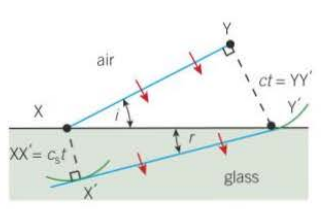
\includegraphics{img/refraction}
\end{center}
The wave front moves
\begin{itemize}
    \item A distance $ct$ at speed $c$ in vacuum from $Y$ to $Y'$.
    \item A distance $c_st$ at speed $c_s$ in the substance from $X$ to $X'$.
\end{itemize}

This gives us equations
\begin{align*}
    \begin{cases}
        ct&=XY'\sin i\\
        c_st&=XY'\sin r
    \end{cases}
\end{align*}
Combining the equations give
$$\frac{\sin i}{\sin r}=\frac{c}{c_s}$$
This shows the \textbf{smaller the speed of light} is in a substance, the \textbf{greater the refractive index} of the substance.

Since the \textbf{frequency does not change} when refraction occurs
$$n_s=\frac{c}{c_s}=\frac{\lambda}{\lambda_s}$$

\subsubsection*{Refraction at a Boundary between Two Transparent Substances}

Consider light crossing a boundary from a substance which the speed of light is $c_1$ to one that the speed of light is $c_2$.
\begin{align*}
    \frac{\sin i}{\sin r}&=\frac{c_1}{c_2}\\
    \frac{1}{c_1}\sin i&=\frac{1}{c_2}\sin r\\
    \frac{c}{c_1}\sin i&=\frac{c}{c_2}\sin r\\
    n_1\sin\theta_1&=n_2\sin\theta_2
\end{align*}
which is the equation form of \textbf{Snell's law}.

Note that the refractive index of air is 1.0003, for most purposes can be assumed to be 1.

\subsubsection*{White Light Spectrum}

A \textbf{glass prism} can be used to split a \textbf{beam of white light} from a filament lamp into the colours of the spectrum. The dispersive effect occur because the speed of light in glass \textbf{depends on wavelength}.
\begin{itemize}
    \item White light is composed of light with a \textbf{continuous range of wavelengths}.
    \item The shorter the wavelength in air, the greater the amount of diffraction.
    \item So each colour in the white light beam is \textbf{refracted by a different amount}.
\end{itemize}
